\documentclass[12pt]{article}

% double-spacing
\usepackage{setspace}
\doublespacing

%% line numbers
%% (turn on before submission)
%\usepackage{lineno}
%\linenumbers

% 1 inch margins
\usepackage[margin=1in]{geometry}

% text color
\usepackage{xcolor}

% bold symbols
\usepackage{bm}

% matrices
\usepackage{amsmath}

% images
\usepackage{graphicx}

% links
\usepackage{hyperref}

% bibliography
\usepackage[super]{natbib} % superscripts
\renewcommand{\refname}{} % empty title
\setcitestyle{citesep={,}} % comma separated

% highlight text that needs editing in red
\newcommand{\edit}[1]{{\color{red}{#1}}}
\newcommand{\add}[1]{{\color{red}{[... #1 ...]}}}

\begin{document}

\section*{Target Journal}

\textit{American Journal of Human Genetics}

\noindent\edit{Other ideas: \textit{PLoS Genetics}, \textit{Genetic Epidemiology}}  %, \textit{Nature Genetics}



\section*{Title}

% no more than 3 lines
% each line <= 54 characters (including spaces)
% convey conceptual significance of paper to broad readership

Adjusting for principal components can induce spurious 
associations in genome-wide association studies in admixed populations

\section*{Authors and Affiliations}

Kelsey E. Grinde,$^{1}$* % should I also list UW?
Brian L. Browning,$^{2}$ 
Sharon R. Browning$^{3}$

%% add Lisa, Alex, Tim if we use WHI data

\begin{enumerate}
\item Department of Mathematics, Statistics, and Computer Science, Macalester College, Saint Paul, MN, 55105, USA
\item Division of Medical Genetics, Department of Medicine, University of Washington, Seattle, WA, 98195, USA
\item Department of Biostatistics, University of Washington, Seattle, WA, 98195, USA
\item[*] kgrinde@macalester.edu
\end{enumerate}


\newpage
\section*{Abstract}

% single paragraph
% <= 250 words
% convey conceptual advance and significance of work to broad readership
% brief background of question, description of results, brief summary of significance of findings
% do not cite any references

%% (from IGES submission)
%% currently 249 words
Principal component analysis (PCA) is widely used to control for population structure in genome-wide association studies (GWAS). It has been shown that the top principal components (PCs) typically reflect population structure, but deciding exactly how many PCs to include in GWAS regression models can be challenging. Often researchers will err on the side of including more PCs than may be actually necessary in order to ensure that population structure is fully captured. However, through both analytic results and application to TOPMed whole genome sequence data for 1,888 and 2,676 unrelated African American individuals from the Jackson Heart Study (JHS) and Chronic Obstructive Pulmonary Disease Genetic Epidemiology Study (COPDGene), respectively, we show that adjusting for extraneous PCs can actually induce spurious associations. In particular, spurious associations arise when PCs capture local genomic features, such as regions of the genome with atypical linkage disequilibrium (LD) patterns, rather than genome-wide ancestry. In JHS and COPDGene, we show that careful LD pruning prior to running PCA, using stricter thresholds and wider windows than is often suggested in the literature, can resolve these issues, whereas excluding lists of high LD regions identified in previous studies does not. We also show that the rate of spurious associations can be appropriately controlled in these data when we simply adjust for either the first PC or a model-based estimate of admixture proportions. Our work demonstrates that great care must be taken when using principal components to control for population structure in genome-wide association studies in admixed populations.


\newpage
\section{Introduction}

% succinct
% no subheadings
% present background info necessary to provide biological context for results


%% what is ancestral heterogeneity?
%Admixed populations such as African Americans and Hispanics/Latinos have historically been vastly underrepresented in genome-wide association studies (GWAS) \cite{need2009, bustamante2011, popejoy2016, morales2018, sirugo2019, martin2019}. 
Considerable variability in global ancestry---the genome-wide proportion of genetic material inherited from each ancestral population---has been observed in many studies of admixed populations such as African Americans and Hispanics/Latinos \citep{parra1998, tishkoff2009, bryc2010aa, bryc2010hl, conomos2016}.
It has been widely documented that heterogeneous global ancestry, as with other types of population structure, can lead to spurious associations in genome-wide association studies \citep{GenomicControl, eigenstrat, marchini2004, price2010}. 
In fact, some authors have even cited the ancestral heterogeneity of admixed populations, and the statistical challenges it poses, as one of many reasons why these populations have been historically underrepresented in genome-wide association studies (GWAS) \citep{need2009, bustamante2011, popejoy2016, hindorff2018, manolio2019}.
%% why do we need to adjust for it?  (confounding)
Spurious associations can arise in GWAS in ancestrally heterogeneous populations when global ancestry confounds the association between genotypes and the phenotype of interest (Figure \ref{fig:confounding}). 
This confounding occurs when the genetic variant being tested differs in frequency across ancestral populations (i.e., global ancestry is associated with genotype) and global ancestry also has an effect on the phenotype via, for example, environmental factors or causal loci elsewhere in the genome that differ in frequency across ancestral groups.

%%% Figure 1: Confounding DAG %%%
\begin{figure}[h]
\center
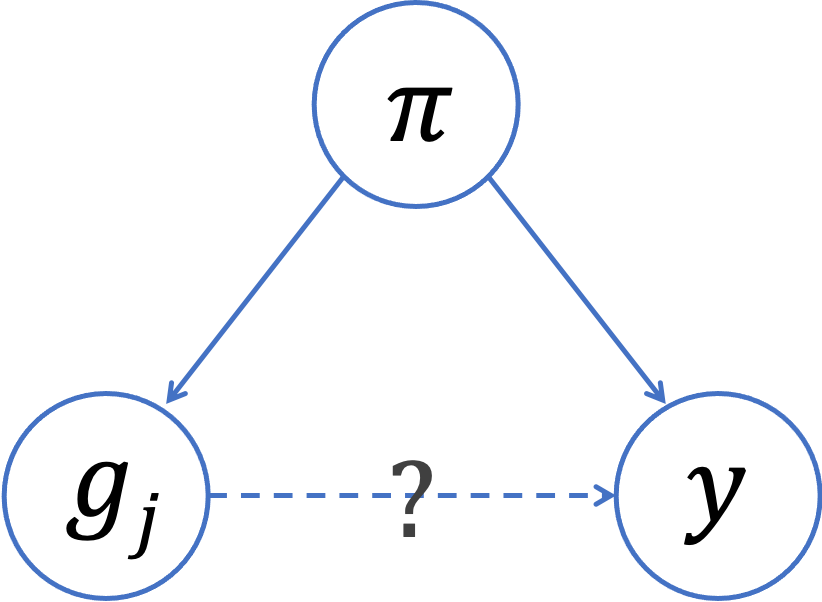
\includegraphics[width=0.4\textwidth]{figs/confounding}
\caption{Global ancestry ($\boldsymbol\pi$) confounds the association between the genotype at position $j$ ($\mathbf{g}_j$) and the phenotype of interest ($\mathbf{y}$) if ancestry is associated with both the genotype (e.g., the allele frequencies differ across the ancestral populations) and the phenotype (e.g., there are environmental or other factors that affect the phenotype and differ across the ancestral populations).}
\label{fig:confounding}
\end{figure}


%% how do we adjust
A number of methods for detecting and controlling for ancestral heterogeneity in genetic association studies have been proposed. 
Early approaches included restricting analyses to subsets of ancestrally homogeneous individuals \citep{lander1994}, performing a genome-wide correction for test statistic inflation due to ancestral heterogeneity via \textit{genomic control} \citep{GenomicControl}, and using family-based designs \citep{tdt}. 
More recently, approaches based on mixed models have been proposed \citep{yu2006, kang2010, yang2014}, using random effects to control for both close (e.g., due to family-based sampling) and distant (e.g., due to shared ancestry) relatedness across individuals.
When studies do not include closely related individuals, a simpler approach is to include inferred global ancestry as a fixed effect in marginal regression models \citep{eigenstrat, pritchard2000}. 
This fixed effects adjustment for global ancestry is currently used extensively throughout the literature, with global ancestry inferred using either model-based ancestry inference methods (e.g., \texttt{frappe} \citep{tang2005}, \texttt{STRUCTURE} \cite{structure}, \texttt{ADMIXTURE} \citep{admixture}) or principal component analysis (e.g., \texttt{EIGENSTRAT} \citep{eigenstrat}, \texttt{SNPRelate} \citep{snprelate}, \texttt{PC-AiR} \citep{conomos2015}).

% summarize model-based approaches (SKIP --- don't want to emphasize as much)
%Model-based approaches for global ancestry inference model the probability of observed genotypes given unobserved ancestry and allele frequencies in each ancestral population \citep{structure, tang2005, admixture, finestructure}. 
%Most often, these approaches are used to estimate global ancestry proportions, also known as \textit{admixture proportions}, the estimated proportion of genetic material inherited by each individual from each ancestral population. 
%Once estimated, these global ancestry proportions can then easily be included as covariates in GWAS models to adjust for ancestral heterogeneity.
%One of the challenges of using these model-based approaches to infer global ancestry is that the total number of ancestral populations usually needs to be pre-specified. 
%In addition, many of these model-based approaches are \textit{supervised}, requiring reference panel data from each ancestral population of interest to estimate allele frequencies.
%Furthermore, ancestry inference is typically conducted at a continental level (e.g., African versus European, rather than South European versus North European), so finer levels of population structure could be missed; recent efforts have considered global ancestry inference on a sub-continental scale \citep{finestructure, durand2014}.

%% overview of PCA 
Principal component analysis (PCA) is a widely-implemented unsupervised approach for inferring global ancestry that does not require reference panel data or pre-specification of the number of ancestral populations of interest and is capable of capturing sub-continental structure \citep{novembre2008}. 
To infer global ancestry using PCA, we preform a singular value decomposition of the matrix of standardized genotypes (i.e., $\mathbf{X} = \mathbf{U}\mathbf{D}\mathbf{V}^\top$) or, equivalently, an eigenvalue decomposition of the genetic relationship matrix (i.e., $\mathbf{X}\mathbf{X}^\top = \mathbf{U}\mathbf{D}^2\mathbf{U}^\top$).
%where $\mathbf{X}$ is the $n \times m$ matrix of standardized gentoypes for $n$ individuals at $m$ single nucleotide variants (SNVs).
It has been shown that top eigenvectors, or \textit{principal components} (PCs), $\mathbf{u}_1, \mathbf{u}_2, \dots$ tend to reflect global ancestry \citep{patterson2006, mcvean2009}.
To adjust for ancestral heterogeneity, we choose some number of PCs %(typically on the order of 1--10 \citep{abegaz2019}
to include as covariates in our GWAS regression models. 

%% issues & solutions: choosing P
Determining the number of PCs needed to capture global ancestry can be difficult. 
Numerous techniques have been proposed for selecting this number, including formal significance tests based on Tracy-Widom theory \citep{patterson2006, eigenstrat}, examining inflation factors \citep{reed2015, conomos2016} and/or the proportion of variance explained by each PC \citep{raska2012, reed2015, conomos2016}, comparing PCs to self-reported race/ethnicity \citep{conomos2016}, and keeping PCs that are significantly associated with the trait \citep{reiner2012, daya2019}.
Typically, the number of PCs selected is on the order of 1--10 \citep{abegaz2019}, but in practice it is not uncommon to see applications in which more PCs are used than may actually be necessary to capture global ancestry. 
This could be due in part to work that has suggested that including higher-order PCs can provide the safeguard of removing ``virtually all stratification" \citep{mathieson2012} at the cost of only ``subtle" decreases in power \citep{liu2011}.
%using the same number of PCs as had been used  to prior work in distinct study populations to justify the choice of 10 PCs \citep{liu2012, reed2015}

%% issues & solutions: other atrifacts 
Another challenge that can arise in using PCA to adjust for ancestral heterogeneity involves ensuring that PCs actually reflect global ancestry and not some other features or artifacts of the data. 
Prior work has shown that PCs can capture relatedness across samples \citep{patterson2006, price2010, abdellaoui2013, conomos2015}, array artifacts or other data quality issues \citep{patterson2006, eigenstrat, price2010, weale2010}, and/or small regions of the genome with unusual patterns of linkage disequilibrium (LD) \citep{patterson2006, eigenstrat, wellcome2007, tian2008, price2008, price2010, weale2010, zou2010, laurie2010, abdellaoui2013, prive2020}. 
%\add{what happens if we adjust for PCs that capture LD instead? include here or save for discussion?}
To address this last issue, some authors have suggested running PCA on a reduced subset of variants after first performing \textit{LD pruning}, using a program such as \texttt{PLINK} \citep{plink} to remove variants that are in ``high" LD (e.g., pairwise-correlation $r^2 > 0.2$) with nearby variants  \citep{wellcome2007, fellay2007, novembre2008, yu2008, nelson2008, anderson2010, weale2010, laurie2010, abdellaoui2013, zhang2013, conomos2015, reed2015, galinsky2016, conomos2016, daya2019}, and/or excluding regions of the genome that are known to have extensive, long-ranging, or otherwise unusual patterns of LD \citep{wellcome2007,  fellay2007, novembre2008, price2008, anderson2010, weale2010, raska2012, conomos2016}. 
A list of these previously-identified high LD regions and references that recommend their exclusion is provided in Table \ref{tab:highLD}.
%after first removing regions of the genome that are known to have high or long-range LD (see Table \ref{tab:highLD}) \citep{wellcome2007,  fellay2007, novembre2008, price2008, anderson2010, weale2010, raska2012, conomos2016} and/or performing LD pruning (i.e., using a program such as \texttt{PLINK} \citep{plink} to remove variants that are in high LD) \citep{wellcome2007, fellay2007, novembre2008, yu2008, nelson2008, anderson2010, weale2010, laurie2010, abdellaoui2013, zhang2013, conomos2015, reed2015, galinsky2016, conomos2016, daya2019}. 


\begin{table}
\label{tab:highLD}
\center
\begin{tabular}{crrl}
Chr & Start (bp) & End (bp) & References \\
\hline
chr1   & 48000000     & 52060567   &    \citep{anderson2010, price2008, weale2010} \\
chr2   & 85941853     & 100500000   &    \citep{anderson2010, price2008, weale2010} \\
chr2   & 129600000   & 140000000   &    \citep{price2008, novembre2008, weale2010, raska2012, conomos2016, prive2018} \\
chr2   & 182882739    & 190000000   &    \citep{anderson2010, price2008, weale2010} \\
chr3   & 47500000     & 50000000    &   \citep{anderson2010, price2008, weale2010}  \\
chr3   & 83500000     & 87000000    &   \citep{anderson2010, price2008, weale2010} \\
chr3   & 89000000     &   97500000   &    \citep{price2008, weale2010} \\
chr3   & 163100000    &   164900000   &    \citep{prive2018} \\
chr5   & 44000000     &   51500000    &   \citep{fellay2007, anderson2010, price2008, weale2010} \\
chr5   & 98000000     &  100500000   &    \citep{price2008, weale2010} \\
chr5   & 129000000    &   132000000   &    \citep{anderson2010, price2008, weale2010} \\
chr5   & 135500000    &   138500000   &   \citep{price2008, weale2010} \\
chr6   &  23800000     &   39000000   &    \citep{fellay2007, anderson2010, price2008, novembre2008, weale2010, raska2012, conomos2016, prive2018} \\
chr6   &  57000000     &   64000000   &    \citep{anderson2010, price2008, weale2010}  \\
chr6   & 140000000    &   142500000   &    \citep{anderson2010, price2008, weale2010}  \\
chr7   &  55000000     &   66193285   &    \citep{anderson2010, price2008, weale2010}  \\
chr8   &   6300000      &  13500000   &    \citep{fellay2007, anderson2010, price2008, novembre2008, tian2008, weale2010, raska2012, conomos2016, prive2018} \\
chr8   &  43000000    &    50000000   &    \citep{anderson2010, price2008, weale2010}  \\
chr8   & 112000000    &   115000000    &   \citep{anderson2010, price2008, weale2010} \\
chr10  &  37000000    &    43000000   &    \citep{anderson2010, price2008, weale2010}  \\
chr11   & 45000000    &    57000000   &    \citep{fellay2007, price2008, weale2010} \\
chr11   & 87500000    &    90500000   &    \citep{anderson2010, price2008, weale2010}  \\
chr12   & 33000000    &    40000000   &    \citep{anderson2010, price2008, weale2010} \\
chr12   & 109500000   &    112021663   &    \citep{price2008, weale2010} \\
chr14   & 46600000    &    47500000   &    \citep{prive2018} \\
chr17   & 37800000    &    42000000    &   \citep{novembre2008, conomos2016} \\
chr20   & 32000000   &     34500000    &   \citep{anderson2010, price2008, weale2010}  \\
\end{tabular}
\caption{Regions of the genome with high, long-range, or otherwise unusual patterns of linkage disequilibrium (LD) that are often recommended for exclusion prior to running PCA. This list of regions was generated on the basis of an extensive literature review. Start and end physical (base pair) positions are provided with respect to genome build 36. Also available for download (in builds 36, 37, or 38) at \href{github.com/kegrinde/PCA}{https://github.com/kegrinde/PCA/}.}
\end{table}


%% motivate  our paper
The above-cited suggestions regarding LD pruning and filtering are not universally implemented and the downstream implications of adjusting for PCs that capture features other than global ancestry are not fully understood.
Furthermore, much of this work was conducted in populations of European ancestry, so recommendations on how best to implement principal component-based adjustment for ancestral heterogeneity in admixed populations are lacking. 
% outline rest of paper
In this paper, we investigate the impact of LD filtering and pruning choices, as well as choices of the number of principal components to include in analyses, on genome-wide association studies in admixed populations.
We conduct simulation studies using whole genome sequence data for African American individuals in the Trans-Omics for Precision Medicine (TOPMed) project and provide analytic results to show that including too many PCs can actually induce spurious associations in GWAS, particularly when those extraneous PCs capture local genomic features rather than genome-wide ancestry.  
To conclude, we provide suggestions regarding best practice for appropriately controlling for ancestral heterogeneity in genome-wide association studies in admixed populations.


\section{Material and Methods}

% provide sufficient detail so readers can understand how experiments were performed and procedures can be repeated
% describe any statistical methods employed in study

\subsection{TOPMed Whole Genome Sequence Data}

The Trans-Omics for Precision Medicine (TOPMed) Whole Genome Sequencing Project is an ongoing project sponsored by the National Heart, Lung, and Blood Institute (NHLBI) that is working to collect and analyze whole-genome sequences, other -omics data, and rich phenotypic information for over 100,000 individuals from diverse backgrounds. 
Data are periodically released on dbGaP for analysis by the broader scientific community. 
Our analysis focuses in particular on data from \textit{freeze 4}, released in 2017, and \textit{freeze 5b}, released in 2018.
These two freezes include samples from a large number of contributing studies.
We focus on two such studies: the Jackson Heart Study (JHS) (accession number: phs000964) and the Genetic Epidemiology of Chronic Obstructive Pulmonary Disease Study (COPDGene) (accession number: phs000951).
In total, the freeze 4 JHS data include 3,406 African American individuals and the freeze 5b COPDGene data include 8,742 African American and European American individuals.

\subsection{TOPMed Sequencing and Quality Control}

% sequencing
For TOPMed freezes 4 and 5b, high coverage ($\approx$ 30X) whole genome sequencing was performed by several sequencing centers, with, for the most part, all samples for a given study sequenced at the same center.
Variant discovery, and genotype calling was performed by the TOPMed Informatics Resources Center (IRC) using the \texttt{GotCloud} pipeline \citep{jun2015}.
% QC
Quality control (QC) was performed by a combination of the sequencing centers, IRC, and TOPMed Data Coordinating Center (DCC), and only those samples and variants that passed this QC are included in the VCF files that can be downloaded from dbGaP.
% references
Details on TOPMed QC methods are available in Taliun et al. \citep{taliun2021} and on the TOPMed website: \href{https://www.nhlbiwgs.org/data-sets}{https://www.nhlbiwgs.org/data-sets}.

\subsection{Additional Filtering and Quality Control}

After downloading the JHS and COPDGene data from dbGaP, we performed additional rounds of filtering/QC before proceeding with further analyses.


New outline: 

\begin{itemize}
\item TOPMed data
	%\begin{itemize}
	%\item what is TOPMed
	%\item which studies did we focus on
	%\item how accessed
	%\item who's in it
	%\item freeze 4 sequencing methods (JHS)
	%\item freeze 5b methods (COPDGene)
	%\item ...
	%\end{itemize}
\item QC
	\begin{itemize}
	%\item basic SNP filters
	\item rare variants \add{move this to QC step?}; \add{citations}
	\item missing rates \add{STILL NEED TO IMPLEMENT THIS!!}
	\item relatives; \add{citations}
	\item non-admixed individuals
	\end{itemize}
\item inferring ancestry using PCA
	\begin{itemize}
	\item software
	\item types of pruning/filtering considered
	\item plots we look at (loadings, screeplots, parallel coordinates, etc.)
	\end{itemize}
\item inferring ancestry using ADMIXTURE
	\begin{itemize}
	\item motivation for comparison
	\item recommended pruning/filtering
	\end{itemize}
\item simulation study
	\begin{itemize}
	\item traits
	\item models
	\item evaluation
	\end{itemize}
\item software and data availability
	\begin{itemize}
	\item dbgap
	\item github
	\end{itemize}
\end{itemize}



\subsection{Adjusting for ancestral heterogeneity in  genome-wide association studies}

To perform genome-wide association studies in samples of unrelated admixed individuals, we use marginal regression models, regressing the trait of interest on the genotype at each position across the genome. 
At a given position $j$, we quantify genotype $g_{ij}$ as the number of copies (0, 1, or 2) of some pre-specified allele (e.g., the minor allele) carried by individual $i$ at that position. 
Considering a quantitative trait $y_i$, we fit one linear regression model at each position ($j = 1, \dots, m$): $$E[y_i \mid g_{ij}, \mathbf{z}_i] = \beta_0 + \beta_j g_{ij} + \boldsymbol{\beta}_z \mathbf{z}_i,$$ where $\mathbf{z}_i$ is a vector of additional covariates (e.g., potential confounding variables) that we want to include in the model.
This linear regression model can be replaced with a logistic regression model in the case of a binary trait (e.g., disease status).
In either case, we test for an association between the trait and genotype by testing the null hypothesis $H_0: \beta_j = 0$ at each position $j = 1, \dots, m$.


To adjust for ancestral heterogeneity, we include inferred global ancestry in the vector $\mathbf{z}_i$ of potential confounders in our regression models. We infer global ancestry using one of two techniques: model-based global ancestry inference of principal component analysis.


%% UPDATE: skipping details of model-based GAI
%\subsubsection{Model-based global ancestry inference}
%
%Various model-based approaches have been developed for estimating global ancestry proportions in admixed populations.
%We represent global ancestry via the vector $\boldsymbol{\pi}_i = \begin{pmatrix} \pi_{i1} & \dots & \pi_{iK} \end{pmatrix}^\top$, where $\pi_{ik}$ denotes the genome-wide proportion of genetic material inherited by individual $i$ from ancestral population $k$ and $\sum_{k=1}^K \pi_{ik} = 1$. 
%Note that the total number of ancestral populations, $K$, typically must be pre-specified, and the definition of global ancestry is typically restricted to the autosomes.
%Admixture proportions can be estimated directly using a program such as \texttt{ADMIXTURE} \citep{admixture}, or by calculating the genome-wide average local ancestry (i.e., $\hat\pi_{ik} = \frac{1}{2m} \sum_{j=1}^m a_{ijk}$), where local ancestry $a_{ijk}$---the number of alleles (0, 1, or 2) inherited by individual $i$ from ancestral population $k$ at position $j$---was first inferred using a program such as \texttt{RFMix} \citep{rfmix}.
%To adjust for ancestral heterogeneity, we include $K-1$ of these estimated admixture proportions as covariates in our GWAS regression models: $$E[y_i \mid g_{ij}, \hat{\boldsymbol\pi}_i] = \beta_0 + \beta_j g_{ij} + \beta_{\pi, 1} \hat\pi_{i,1} + \dots + \beta_{\pi, K-1} \hat\pi_{i, K-1}.$$
%
%Many model-based global ancestry inference programs are supervised, requiring data from individuals from each ancestral population of interest to form a reference panel. However, some approaches such as \texttt{ADMIXTURE} can also be run without a reference panel.

%% UPDATE: moved most of this to intro
%\subsubsection{Principal component analysis}
%
%Principal component analysis (PCA) is an unsupervised dimension-reduction technique that is widely used for inferring population structure in genetic studies, with a number of software programs available for running PCA on genotype or sequence data (e.g., \texttt{EIGENSTRAT} \citep{eigenstrat}, \texttt{SNPRelate} \citep{snprelate}, \texttt{PC-Air} \citep{conomos2015}).
%To run PCA, we perform a singular value decomposition of the matrix of standardized genotypes (i.e., $\mathbf{X} = \mathbf{UDV}^\top$) or, equivalently, an eigenvalue decomposition of the genetic relationship matrix (i.e., $\mathbf{XX}^\top = \mathbf{UD}^2\mathbf{U}^\top$). 
%The top principal components ($\mathbf{u}_1, \mathbf{u}_2, \dots$) typically capture global ancestry \citep{patterson2006, mcvean2009}. 
%To adjust for ancestral heterogeneity, we choose some number of principal components, $P$, needed to capture global ancestry (typically $1 \le P << n$) and include those PCs as covariates in our GWAS regression models: $$E[y_i \mid g_{ij}, u_{i1}, \dots, u_{iP}] = \beta_0 + \beta_j g_{ij} + \beta_{u 1} u_{i1} + \dots + \beta_{u P} u_{i P}.$$
%A number of techniques have been proposed for selecting the number of PCs, $P$, including formal significance tests based on Tracy-Widom theory \citep{patterson2006, eigenstrat}, examining the proportion of variance explained by each PC \citep{reed2015}, comparing PCs to self-reported ancestry \citep{conomos2016}, and/or keeping PCs that are significantly associated with the trait \citep{reiner2012, daya2019}. 



%% UPDATE: moved most of this to intro
%\subsubsection{Variant- and sample-level filtering}
%It is often recommended that filtering be performed at the variant and/or sample level prior to inferring global ancestry. 
%Prior work has shown that both model-based estimates of global ancestry \add{cite Tim's GAW paper} and principal components \citep{conomos2015, eigenstrat, patterson2006} \add{check patterson, maybe add more refs: Price 2010} can reflect family structure and/or cryptic relatedness rather than global ancestry when a sample includes related individuals, but restricting analyses to a subset of unrelated individuals (e.g., using the iterative procedure proposed by \cite{conomos2016related}) can circumvent that issue. 
%At the variant level, it is common to perform filtering based on minor allele frequency \add{find references}, as prior work has shown that methods such as \texttt{EIGENSTRAT} can perform poorly when applied to rare variants \citep{kirk2016}.
%
%Other variant-level filters have been recommended to address the sensitivity of model-based and PCA approaches to the presence of linkage disequilibrium (LD).
%This can include \textit{LD pruning}, using a program such as \texttt{PLINK} \add{CITE} to remove variants that are ``highly" correlated (e.g., pairwise-correlation $r^2 > 0.2$) with nearby variants (e.g., within a window of size \edit{??}) \add{\citep{admixture}, ADD MORE}, and/or excluding regions of the genome that are known to have extensive, long-ranging, or otherwise unusual patterns of LD \add{CITE}. 
%A list of previously-identified high LD regions is provided in Appendix \edit{??}. 
%\add{say something about how not everyone does this, it's not always clear which parameters should be used, and/or much of this work has been performed in European pop and not clear what should be done in admixed pop}


%\add{Add missing rates (SNPs and people) here? Or just frame as QC step?)}


\subsection{Simulation study using TOPMed whole genome sequence data}

\edit{Are we sure we want to use TOPMed? Or should we switch back to WHI?}

We implement a simulation study using whole genome sequence data from the Trans-Omics for Precision Medicine (TOPMed) program to compare different approaches for adjusting for ancestral heterogeneity and explore the impact of different variant-level filtering choices, particular with respect to linkage disequlibrium. 

\subsubsection{TOPMed whole genome sequence data}

TOPMed is \add{describe TOPMed}.
Whole genome sequence data for contributing TOPMed studies is available on dbGaP. 
We focus on two such studies, the Jackson Heart Study (JHS) (accession number: phs000964) and the Chronic Obstructive Pulmonary Disease Genetic Epidemiology Study (COPDGene) (accession number: phs000951).

\edit{
\begin{itemize}
\item describe TOPMed 
\item describe sequencing methods
\item how many samples in each study
\end{itemize}
}

\subsubsection{Quality control}

% variant-level filters
We process the sequence data for quality control, keeping only those variants that are bi-allelic, have a minor allele count of at least one, and pass standard variant filters (Mendelian or duplicate genotype discordance $< 3/5\%$, Hardy-Weinberg Equilibrium p-value $> 1 \times 10^{-6}$, etc.).
\add{Add filter for missing rates!}
After all exclusions, we are left with \edit{???} and \edit{???} variants in JHS and COPDGene, respectively.

% sample-level filters
After variant-level filtering, we then use the iterative procedure suggested by Conomos et al. \citep{conomos2016} and implemented in the \edit{TOPMed analysis pipeline} to identify a subset of \edit{??} mutually unrelated individuals. 
\add{more details about iterative procedure; e.g., sing a kinship threshold of \edit{0.044 $\leftarrow$ double-check} (i.e., excluding first, second, and third degree relatives)} 
Next, we run an unsupervised \texttt{ADMIXTURE} analysis with $K = 2$ and $K = 3$ and plot inferred global ancestry proportions to identify admixed (African American) and non-admixed (European) individuals.
\add{more details about thresholds used}
After sample-level filtering,  \edit{???} and \edit{???} individuals remain in JHS and COPDGene, respectively.




\textbf{QC for JHS} (dbgap accession phs000964):

\begin{itemize}
\item filtering
	\begin{itemize}
	\item bi-allelic SNPs
	\item minor allele count at least 1
	\item pass variant filters (in VCFs that were downloaded from dbgap): overlaps with SNP, overlaps with indel, overlaps with VNTR, failed SVM filter, high (3/5\% or more) mendelian or duplicate genotype discordance, excess heterozygosity with HWE p-value < 1e-6
	\end{itemize}
\item merge the two subsets (cg1 and cg3)
\item convert from VCF to GDS
\item remove close relatives
	\begin{itemize}
	\item run king (LD r threshold: 0.32, LD window size: 10, MAF threshold: 0.01, exclude PCA corr: TRUE, build: hg19)
	\item run PC-AiR 
	\item run PCRelate 
	\item run PC-AiR again
	\item run PCRelate again
	\end{itemize}
\item find African Americans
	\begin{itemize}
	\item run stricter LD pruning (MAF  = 0.01, window size = 0.5, rsq = 0.01, regions = TRUE, build 37)
		\begin{itemize}
		\item List of regions stored here: \verb"/projects/browning/brwnlab/kelsey/spurious_assoc/highLD_regions/"
		\end{itemize}
	\item convert GDS to BED
	\item run ADMIXTURE (K = 2 and K = 3)
	\item plot proportions
	\item exclude 40 people inferred to be 100\% European; left with 1888
	\end{itemize}
\end{itemize}

\textbf{QC for COPDGene} (phs000951):

\begin{itemize}
\item filtering
	\begin{itemize}
	\item bi-allelic SNPs
	\item minor allele count at least 1
	\item pass filtering (from GDS annotation info, I inferred this to include: variant located in centromeric region, variant failed SVM filter, mendelian or duplicate genotype discordance is high (3/5\% or more), excess heterozygosity in chrX in males, excess heterozygosity with HWE p-value < 1e-6)
	\end{itemize}
\item convert from VCF to GDS
\item remove close relatives
	\begin{itemize}
	\item run king (LD r threshod = 0.32, LD window size = 10, MAF threshodl = 0.01, exclude PCA corr = TRUE, build = hg38); regions =         see table below
	\item run PCAiR
	\item run PCRelate
	\item run PCAiR again
	\end{itemize}
\item find African Americans
	\begin{itemize}
	\item run stricter LD pruning (exclude PCA corr regions = TRUE, build = hg38, LD R threshold = 0.1, LD window size = 10, MAF threshold = 0.01); regions = \verb"/projects/browning/brwnlab/kelsey/spurious_assoc/highLD_regions/"
	\item convert from GDS to PLINK
	\item run ADMIXTURE with K = 2 and K = 3
	\item plot proportions and use cut-off of 30\% to identify (and then remove) Europeans : Parker et al. 2014 "Admixture mapping identifies a quantitative trait locus associated with..." \verb"https://www.ncbi.nlm.nih.gov/pmc/articles/PMC4190160/" (reduced from 8406 to 2676)
	\end{itemize}
\end{itemize}

\begin{table}
\begin{tabular}{ccccc}
name & chrom & start.base  & end.base  & comment \\
2q21    &  2  &  129883530 & 140283530       &  LCT \\
HLA      &    6 &   24092021  & 38892022 & includes MHC \\
8p23  &        8   &  6612592 &  13455629 &   inversion \\
17q21.31 &    17  &  40546474 & 44644684   &  inversion \\
\end{tabular}
\caption{TOPMed hg19 high corr regions}
\end{table}

\begin{table}
\begin{tabular}{ccccc}
name & chrom & start.base  & end.base  & comment \\
2q21    &  2  &  129125957 & 139525961       &  LCT \\
HLA      &    6 &   24091793  & 38924246 & includes MHC \\
8p23  &        8   &  6755071 &  13598120 &   inversion \\
17q21.31 &    17  &  42394456 & 46567318   &  inversion \\
\end{tabular}
\caption{TOPMed hg38 high corr regions}
\end{table}

\subsubsection{Genetic ancestry inference}

\begin{itemize}
\item ADMIXTURE
	\begin{itemize}
	\item JHS: ran with both K = 2 and K = 3
	\item COPDGene: ran with both K = 2 and K = 3
	\item unsupervised for both
	\end{itemize}
\item PCA using SNPRelate
\item what filtering was performed, and how many variants left after filtering
	\begin{itemize}
	\item JHS, ADMIXTURE: see above
	\item JHS, PCA: exclude regions (TRUE/FALSE), r-squared (1, 0.1, 0.2, 0.05), window size (0, 0.5, 10), and MAF (0, 0.01) 
		\begin{itemize}
		\item no filtering: FALSE-1-0-0
		\item MAF filtering: FALSE-1-0-0.01
		\item exclude but no prune: TRUE-1-0-0.01
		\item prune but no exclude: FALSE-0.1-0.5-0.01 and FALSE-0.1-10-0.01 and FALSE-0.2-0.5-0.01 and FALSE-0.05-0.5-0.01
		\item prune and exclude: TRUE-0.1-0.5-0.01 and TRUE-0.1-10-0.01 and TRUE-0.2-0.5-0.01 and TRUE-0.05-0.5-0.01
		\end{itemize}
	\item COPD, ADMIXTURE: see above
	\item COPD, PCA: exclude regions (TRUE/FALSE), r-squared (1, 0.1, 0.2, 0.05), window size (0, 0.5, 10), MAF (0, 0.01)
		\begin{itemize}
		\item no filtering: FALSE-1-0-0
		\item MAF filtering: FALSE-1-0-0.01
		\item exclude but no prune: TRUE-1-0-0.01
		\item prune but no exclude: FALSE-0.1-0.5-0.01, FALSE-0.1-10-0.01, FALSE-0.2-0.5-0.01, FALSE-0.05-0.5-0.01
		\item prune and exclude: TRUE-0.1-0.5-0.01, TRUE-0.1-10-0.01, TRUE-0.05-0.5-0.01, TRUE-0.2-0.5-0.01
		\end{itemize}	
	\item COPD, also ran SNPRelate on Europeans with different levels of filtering (FALSE-0.1-0.5-0.01, FALSE-0.2-0.5-0.01, FALSE-1-0-0.01, FALSE-1-0-0, TRUE-0.1-0.5-0.01, TRUE-0.2-0.5-0.01, TRUE-1-0-0.01)
	\end{itemize}
\end{itemize}


\subsubsection{Evaluating population structure adjustment approaches}

\begin{itemize}
\item plot PCs vs global ancestry proportions
\item plot SNP loadings 
\end{itemize}


\begin{itemize}
\item simulating traits (effect sizes, choice of causal SNPs)
	\begin{itemize}
	\item find loading peaks from "naive" approach
	\item simulate trait that is beta * x + rnorm(0, 1), where beta = 1 or 2 and x = genotype at one of the peaks
	\end{itemize}
\item running GWAS
	\begin{itemize}
	\item for each of 188*2 simulated phenotypes
	\item for each set of PCs
	\item including 1, 4, or 10 PCs
	\end{itemize}
\item defining spurious associations
\end{itemize}



\section{Results}

\subsection{Ancestral heterogeneity in TOPMed African American samples}

\begin{itemize}
\item quickly summarize ancestral heterogeneity (barplots of ADMIXTURE proportions)
\end{itemize}


\subsection{Confirming the importance of adjusting for population structure}

\begin{itemize}
\item show an example manhattan plot with no adjustment
\item compare average number of spurious associations
\item tie in theoretical results
\end{itemize}

\subsection{Comparing different approaches for adjusting for population structure}

Part 1: how does FWER compare?

\begin{itemize}
\item manhattan plots for one or two simulated traits
\item overall summary of rejection rates
\item is it appropriate to use same significance threshold for all?
\end{itemize}

\noindent Part 2: how does rate of spurious associations compare? (and alpha-adjusted spurious assoc?)

\begin{itemize}
\item manhattan plots for one or two traits
\item overall summary of rejection rates
\end{itemize}

\noindent Part 3: why is this happening?

\begin{itemize}
\item are admixture proportions and PCs capturing similar information?
	\begin{itemize}
	\item correlation between PCs and admixture proportions (PC1 highly correlated with admix prop)
	\item correlation between PCs and genotypes (without pruning, later PCs highly correlated with genotypes in small regions)
	\end{itemize}
\item mathematical results
\end{itemize}


%\subsection{Power}
%
% skip this for now
%
% Do they have similar power?


\section{Discussion}

% explain significance of results and place them in broader context
% may contain subheadings

Global ancestry = confounder
\begin{itemize}
\item Summarize conditions under which global ancestry is a confounder 
\item Relate to current understanding in literature
\end{itemize}

\noindent Be careful with PCs!
\begin{itemize}
\item Summarize conditions under which PCs can be problematic
\item Relate to current understanding in literature (what have others shown can happen if you include a PC that captures local LD? how are things different in admixed populations, where LD is more extensive?)
\item Relate to concept of collider bias
\item Suggested diagnostics
\end{itemize}

% GWAS vs admixture mapping

% sequence vs genotype data

% how does this apply to mixed models?


\newpage
\section{Appendices}

% can put detailed results of statistical analyses here
% may contain subheadings

\subsection{Regions Removed Prior to PCA}

\begin{itemize}
\item a list of all "high-LD" regions removed prior to running PCA
\end{itemize}

\subsection{Mathematical Derivations}

\begin{itemize}
\item theoretical results
\item proofs
\item simulations validating theory
\end{itemize}


\newpage
\section*{Supplemental Data}

% briefly list what types of data are included in supplemental data (a separate PDF document)
% e.g., "Supplemental Data include four figures and two tables"

Supplemental Data include \add{??} figures and \add{??} tables.



\section*{Declaration of Interests}

% We ask that you and all authors disclose any personal financial interests (examples include stocks or shares in companies with interests related to the submitted work or consulting fees from companies that could have interests related to the work), professional affiliations, advisory positions, board memberships, or patent holdings that are related to the subject matter of the contribution. As a guideline, you need to declare an interest for (1) any affiliation associated with a payment or financial benefit exceeding $10,000 p.a. or 5% ownership of a company or (2) research funding by a company with related interests. You do not need to disclose diversified mutual funds, 401ks, or investment trusts.
% https://www.cell.com/declaration-of-interests

The authors declare no competing interests.


\section*{Acknowledgments}

% contributions from nonauthors
% list funding sources
% add any necessary data-related acknowledgments

K.E.G. was supported by the National Science Foundation Graduate Research Fellowship Program under grant no. DGE-1256082. Any opinions, findings, and conclusions or recommendations expressed in this material are those of the author(s) and do not necessarily reflect the views of the National Science Foundation.



\section*{Web Resources}

%list and provide URL for any web-based resources (e.g., datbase, online computer programs, etc.)
%For all computer programs, please provide a URL for the website at which the computer program described in the manuscript will be made publicly available.

\edit{GitHub Repository: lists of regions to exclude, code for LD pruning, excluding, and plotting loadings}


\section*{Data and Code Availability}

%statement describing the availability of new datasets and/or code associated with the paper.
%includes any conditions for access of datasets and/or code not publicly available.
%also include any accession numbers, DOIs or unique identifiers, or web links to deposited datasets

%%examples
%The [datasets/code] generated during this study are available at [name of repository] [accession code/web link].
%The published article includes all [datasets/code] generated or analyzed during this study.
%This study did not generate/analyze [datasets/code].
%There are restrictions to the availability of [dataset/code] due to [reason for restrictions].
%Original/source data for [figures/datatype] in the paper is available [e.g., Mendeley Data DOI].
%The [datasets/code] supporting the current study have not been deposited in a public repository because [reason data are not public] but are available from the corresponding author on request.

\newpage
\section*{References}

%include only articles that are published.
%"et al." should be used only after 10 authors.
%Please use the following styles for references:

%%Article in a periodical
%1. Leach, N.T., Sun, Y.,Michaud, S., Zheng, Y., Ligon, K.L., Ligon, A.H., Sander, T., Korf, B.R., Lu, W., Harris, D.J., et al. (2007). Disruption of diacylglycerol kinase delta (DGKD) associated with seizures in humans and mice. Am. J. Hum. Genet. 80, 792–799.

%%Article in a book
%2. King, S.M. (2003). Dynein motors: Structure, mechanochemistry and regulation. In Molecular Motors, M. Schliwa, ed. (Wiley-VCH Verlag GmbH), pp. 45–78.

%%Entire book
%3. Cowan, W.M., Jessell, T.M., and Zipursky, S.L. (1997). Molecular and Cellular Approaches to Neural Development (Oxford University Press).

%%Online reference
%4. Rothwarf, D.M., and Karin, M. (1999). The NF-kB pathway: a paradigm in information transfer from membrane to nucleus. Science’s STKE, http://www.stke.org/cgi/content/full/OC_sigtrans;1999/5/rel.

%%Computer program
%5. Hubbard, S.J. and Thornton, J.M. (1993). NACCESS computer program (Department of Biochemistry and Molecular Biology, University College London).
% Software may also be cited in text; for an in-text citation, include the name of the manufacturer in parentheses.

%%Dissertation/Thesis
%6. Smith, J.P. (1985). DNA sequences. PhD thesis (Massachusetts Institute of Technology).

%The current AJHG reference format for Endnote users can be downloaded from http://www.endnote.com/support/enstyles.asp
%The current AJHG reference format for RefMan users can be downloaded from http://www.refman.com/support/rmstyles.asp

%%In-Text Citations
%Unpublished data, abstracts, and personal communications may be cited within the text only. Submitted articles that have not yet been accepted should be cited as data not shown, unpublished data, or a personal communication.
%Unpublished data may refer only to work from an author of the manuscript being submitted.
%A personal communication should be documented by a letter of permission (this may be in the form of an e-mail communication, letter, or other appropriate form of permission).
%Please use the following style for such citations:

%%Unpublished data 
%(M.A., unpublished data)

%%Abstract
%(M. Adams et al., 1997, Soc. Neurosci., abstract)

%%Personal communication
%(M. Adams, personal communication) 

\bibliographystyle{ajhg}
\bibliography{spurious}


\newpage
\section*{Figure Titles and Legends}

% brief title describing entire figure without citing specific panels
% subsequent description of each panel

% numbered consecutively with whole numbers (e.g., Figure 1, Figure 2, etc. rather than Figure 1a, Figure 1b, etc.)

% figures may not exceed one page

% figure titles may not contain parenthetical information, reference citations, or footnotes

% all reference citations within a figure must also be included in the figure legend

%For any figures presenting pooled data, the measures should be defined in the figure legends (for example, data are represented as the mean ± SEM).

%%https://www.cell.com/figureguidelines


\section*{Tables}

%Include tables in the submitted manuscript after the figure titles and legends. Tables should not be saved as figures, i.e., as .jpg or .tif files. All tables intended for print should be incorporated into the end of the manuscript Word file. Tables should not be uploaded individually.

%When creating a table, please use the Microsoft Word table function, and please do not place an Excel table into a Word document. Tables not created with the Microsoft Word table function will be sent back for revision. Do not submit a table in PDF format.

%Word tables should not be tab or space delineatedand and should not include colored text or shading, but embedded graphics with color are OK.

%Do not use paragraph returns to separate data within a cell.

%Tables should include a title, and footnotes and/or legends should be concise. 

%Table titles may not contain parenthetical information, reference citations, or footnote citations.

%Use superscripted lowercase letters (beginning with “a”) for footnotes in tables. Do not use numbers or symbols.

%Tables must be numbered as Table 1, Table 2, Table 3, etc., rather than as Table 1a, Table 1b, Table 1c, etc.

%If italic font is used within a table to indicate some feature of the data, an explanation of its meaning must be given in the table legend. Bold text may not be used in tables.

%If a referenced paper or study is mentioned within a table, it must be included in the References list and must be followed by its appropriate citation number (e.g., “Author et al.1”) within the table.

%All abbreviations within a table must be defined in the table legend or footnotes.

\end{document}